\documentclass{beamer}

\usetheme{Madrid} % You can choose any theme you prefer

% Packages for enhanced functionality
\usepackage{graphicx}
\usepackage{caption}
% Load necessary TikZ libraries
\usepackage{tikz}
\usetikzlibrary{shapes.geometric, arrows}

% Define styles for flowchart
\tikzstyle{startstop} = [
    rectangle, 
    rounded corners, 
    minimum width=3cm, 
    minimum height=1cm,
    text centered, 
    draw=black, 
    fill=red!30
]

\tikzstyle{process} = [
    rectangle, 
    minimum width=3cm, 
    minimum height=1cm, 
    text centered, 
    draw=black, 
    fill=orange!30
]

\tikzstyle{decision} = [
    diamond, 
    minimum width=3cm, 
    minimum height=1cm, 
    text centered, 
    draw=black, 
    fill=green!30
]

\tikzstyle{arrow} = [
    thick, 
    ->, 
    >=stealth
]

\usepackage{amsmath, amssymb}
\usepackage{booktabs}

% Title and Author Information
\title{Online Geometric Optimization in the Bandit Setting\\Against an Adaptive Adversary}
\author{H. Brendan McMahan and Avrim Blum}
\institute{Carnegie Mellon University}
\date{\today}

\begin{document}

\maketitle

\section{Introduction}

\begin{frame}
\frametitle{Introduction}
\begin{columns}
    \column{0.6\textwidth}
    \begin{itemize}
        \item Overview of online optimization in adversarial environments.
        \item Importance of studying bandit settings with limited feedback.
        \item Addressing challenges posed by adaptive adversaries.
    \end{itemize}
    \column{0.4\textwidth}
    % \includegraphics[width=\textwidth]{images/online_optimization.png} % Replace with your image path
\end{columns}
\end{frame}

\begin{frame}
\frametitle{Context: Online Optimization with an Adversary}
\begin{columns}
    \column{0.6\textwidth}
    \begin{itemize}
        \item Online optimization involves making sequential decisions.
        \item Adversaries can influence the environment by selecting cost vectors.
        \item Applications in machine learning, economics, and network routing.
    \end{itemize}
    \column{0.4\textwidth}
    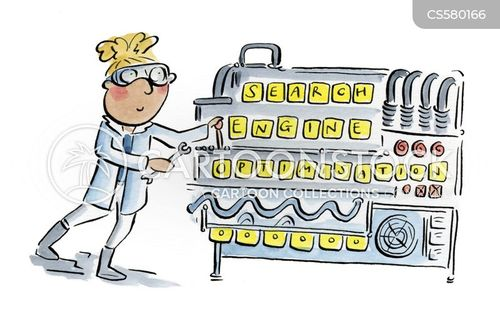
\includegraphics[width=\textwidth]{images/adversary_context.jpg} % Replace with your image path
\end{columns}
\end{frame}

\begin{frame}
\frametitle{Objective: Solving the Bandit Version}
\begin{columns}
    \column{0.6\textwidth}
    \begin{itemize}
        \item Transition from full-information to bandit feedback.
        \item Challenges due to limited information after each decision.
        \item Goal: Develop algorithms that perform well despite these limitations.
    \end{itemize}
    \column{0.4\textwidth}
    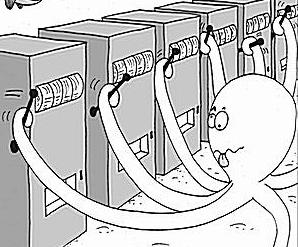
\includegraphics[width=\textwidth]{images/bandit_setting.jpg} % Replace with your image path
\end{columns}
\end{frame}

\section{Key Problem Setup}

\begin{frame}
\frametitle{Description of the Online Optimization Problem}
\begin{itemize}
    \item Set of feasible points \( S \subset \mathbb{R}^n \).
    \item Sequential decision-making over \( T \) rounds.
    \item At each round \( t \), select \( x_t \in S \) and incur cost \( c_t \cdot x_t \).
\end{itemize}
\begin{exampleblock}{Mathematical Example}
    \textbf{Example:} Let \( S \) be the unit simplex in \( \mathbb{R}^n \), i.e.,
    \[
    S = \left\{ x \in \mathbb{R}^n \mid x_i \geq 0 \text{ for all } i, \sum_{i=1}^n x_i = 1 \right\}
    \]
    This setup is common in online portfolio selection.
\end{exampleblock}
\end{frame}

\begin{frame}
\frametitle{Adversary and Algorithm Interactions}
\begin{columns}
    \column{0.6\textwidth}
    \begin{itemize}
        \item Adversary selects cost vectors \( c_t \in \mathbb{R}^n \).
        \item Algorithm selects decisions \( x_t \in S \) without knowing \( c_t \) in advance.
        \item Objective is to minimize cumulative cost over \( T \) rounds.
    \end{itemize}
    \column{0.4\textwidth}
    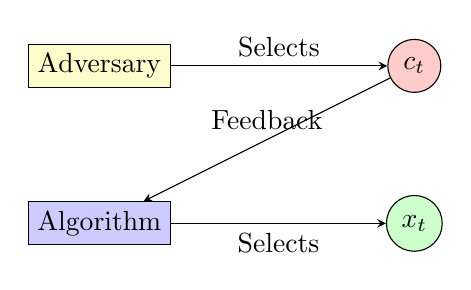
\begin{tikzpicture}[>=stealth, node distance=2cm]
        \node (adversary) [draw, rectangle, fill=yellow!20] {Adversary};
        \node (algorithm) [draw, rectangle, below of=adversary, fill=blue!20] {Algorithm};
        \node (cost) [draw, circle, right of=adversary, xshift=2cm, fill=red!20] {$c_t$};
        \node (decision) [draw, circle, right of=algorithm, xshift=2cm, fill=green!20] {$x_t$};
        
        \draw[->] (adversary) -- (cost) node[midway, above] {Selects};
        \draw[->] (algorithm) -- (decision) node[midway, below] {Selects};
        \draw[->] (cost) -- (algorithm) node[midway, above] {Feedback};
    \end{tikzpicture}
\end{columns}
\end{frame}

\section{Online Optimization Problem}

\begin{frame}
\frametitle{Set \( S \subset \mathbb{R}^n \)}
\begin{itemize}
    \item \( S \) represents all possible feasible decisions.
    \item Geometric properties of \( S \) influence algorithm design.
    \item Examples: Convex sets, polytopes, or combinatorial structures.
\end{itemize}
\begin{exampleblock}{Mathematical Example}
    \textbf{Convex Set:} Let \( S = \{ x \in \mathbb{R}^n \mid \|x\|_2 \leq 1 \} \) be the unit ball in \( \mathbb{R}^n \). This convex set allows the use of gradient-based optimization methods due to its smooth boundary.
\end{exampleblock}
\end{frame}

\begin{frame}
\frametitle{Cost Incurred: \( c_t \cdot x_t \)}
\begin{itemize}
    \item Inner product representing the cost for decision \( x_t \).
    \item \( c_t \) is the cost vector chosen by the adversary.
    \item Objective: Minimize the sum \( \sum_{t=1}^T c_t \cdot x_t \).
\end{itemize}
\begin{equation*}
    \text{Total Cost} = \sum_{t=1}^T c_t \cdot x_t
\end{equation*}
\end{frame}

\section{Offline Optimization Problem}

\begin{frame}
\frametitle{The Role of an Oracle for Offline Optimization}
\begin{itemize}
    \item Oracle solves \( \min_{x \in S} \left( c \cdot x \right) \) efficiently.
    \item Assumes full knowledge of cost vectors.
    \item Serves as a benchmark for online algorithms.
\end{itemize}
\begin{exampleblock}{Mathematical Example}
    \textbf{Offline Optimization:} Given all cost vectors \( \{c_1, c_2, \dots, c_T\} \) in advance, the oracle solves:
    \[
    \min_{x \in S} \sum_{t=1}^T c_t \cdot x
    \]
    This provides the best possible cumulative cost.
\end{exampleblock}
\end{frame}

\begin{frame}
\frametitle{Objective: \( \min_{x \in S} \left( c \cdot x \right) \)}
\begin{itemize}
    \item Offline problem assumes all cost vectors are known in advance.
    \item Provides the optimal benchmark for comparison.
    \item Online algorithms aim to perform nearly as well without this knowledge.
\end{itemize}
\begin{equation*}
    \text{Optimal Offline Cost} = \min_{x \in S} \sum_{t=1}^T c_t \cdot x
\end{equation*}
\end{frame}

\section{Bandit Version of the Problem}

\begin{frame}
\frametitle{Observing Only the Cost: \( c_t \cdot x_t \)}
\begin{itemize}
    \item Limited feedback: Only the incurred cost is observed.
    \item No access to the full cost vector \( c_t \).
    \item Necessitates exploration to gather information.
\end{itemize}
\begin{exampleblock}{Concrete Example}
    \textbf{Example:} In online advertising, selecting an ad (decision \( x_t \)) and only observing the click-through rate (incurred cost) without knowing the underlying user preferences (cost vector \( c_t \)).
\end{exampleblock}
\end{frame}

\begin{frame}
\frametitle{Example: Online Shortest Path Problem}
\begin{columns}
    \column{0.6\textwidth}
    \begin{itemize}
        \item Decision set \( S \) consists of all possible paths in a network.
        \item Cost vectors represent edge weights chosen by the adversary.
        \item Feedback is the total cost of the chosen path only.
    \end{itemize}
    \begin{exampleblock}{Concrete Example}
        Consider a network with 4 nodes (A, B, C, D) and 5 edges. At each round, an adversary assigns weights to the edges. The algorithm selects a path from node A to node D and only observes the sum of the weights on the chosen path.
    \end{exampleblock}
    \column{0.4\textwidth}
    % \includegraphics[width=\textwidth]{images/shortest_path_example.png} % Replace with your image path
\end{columns}
\end{frame}

\section{Adversaries: Oblivious vs. Adaptive}

\begin{frame}
\frametitle{Difference Between Oblivious and Adaptive Adversaries}
\begin{columns}
    \column{0.6\textwidth}
    \begin{itemize}
        \item \textbf{Oblivious Adversary}: Chooses all cost vectors in advance.
        \item \textbf{Adaptive Adversary}: Chooses \( c_t \) based on past algorithm decisions.
        \item Adaptive adversaries are more powerful and challenging.
    \end{itemize}
    \column{0.4\textwidth}
    \begin{table}[h]
    \centering
    \begin{tabular}{|c|c|c|}
    \hline
    \textbf{Adversary Type} & \textbf{Description} & \textbf{Challenge} \\ \hline
    Oblivious & Chooses all \( c_t \) in advance & Fixed cost structure \\ \hline
    Adaptive & Chooses \( c_t \) based on past \( x_s \) & Dynamic cost structure \\ \hline
    \end{tabular}
    \caption{Comparison of Adversary Types}
    \end{table}
\end{columns}
\end{frame}

\begin{frame}
\frametitle{Impact of Adversary's Strategy on the Algorithm}
\begin{columns}
    \column{0.6\textwidth}
    \begin{itemize}
        \item Adaptive strategies can exploit algorithm's weaknesses.
        \item Necessitates robust algorithms that can handle changing environments.
        \item Importance of maintaining low regret despite adversary's adaptability.
    \end{itemize}
    \column{0.4\textwidth}
    % \includegraphics[width=\textwidth]{images/adaptive_adversary.png} % Replace with your image path
\end{columns}
\end{frame}

\section{Regret in the Context of Online Optimization}

\begin{frame}
\frametitle{Formal Definition of Regret}
\begin{itemize}
    \item \textbf{Regret} measures the performance gap between the algorithm and the best offline decision.
    \item Mathematically: 
    \[
    \text{Regret} = \mathbb{E}\left[\sum_{t=1}^T c_t \cdot x_t \right] - \mathbb{E}\left[\min_{x \in S} \sum_{t=1}^T c_t \cdot x \right]
    \]
    \begin{itemize}
        \item \( \mathbb{E} \): Expectation over the algorithm's randomness.
        \item \( c_t \): Cost vector at round \( t \).
        \item \( x_t \): Decision made by the algorithm at round \( t \).
    \end{itemize}
    \item Goal is to achieve sublinear regret: \( \text{Regret} = o(T) \).
\end{itemize}
\end{frame}

\begin{frame}
\frametitle{Goal: Minimize Regret}
\begin{columns}
    \column{0.6\textwidth}
    \begin{itemize}
        \item Achieve sublinear regret: \( \text{Regret} = o(T) \).
        \item Ensures average regret per round goes to zero as \( T \) increases.
        \item Fundamental objective in online learning and optimization.
    \end{itemize}
    \column{0.4\textwidth}
    % \includegraphics[width=\textwidth]{images/regret_convergence.png} % Replace with your image path
\end{columns}
\end{frame}

\section{Kalai-Vempala Algorithm}

\begin{frame}
\frametitle{Description of the Kalai-Vempala Algorithm}
\begin{itemize}
    \item General algorithm for online convex optimization.
    \item Utilizes the exponential weights framework.
    \item Assumes full feedback: Observes entire cost vector \( c_t \) after each decision.
\end{itemize}
\begin{exampleblock}{Mathematical Formulation}
    The Kalai-Vempala algorithm updates the weight \( w_t(x) \) for each decision \( x \in S \) as:
    \[
    w_{t+1}(x) = w_t(x) \exp\left(-\eta c_t \cdot x \right)
    \]
    where \( \eta \) is the learning rate.
\end{exampleblock}
\end{frame}

\begin{frame}
\frametitle{Assumption: Adversary Selects Cost Vectors After Decision}
\begin{itemize}
    \item The algorithm selects \( x_t \) without knowing \( c_t \).
    \item After selection, \( c_t \) is revealed.
    \item Enables the use of gradient-based updates in the algorithm.
\end{itemize}
\begin{equation*}
    x_t = \frac{w_t(x)}{\sum_{x' \in S} w_t(x')}
\end{equation*}
\end{frame}

\section{Adaptive Adversary and Bandit Setting}

\begin{frame}
\frametitle{Transition to the Bandit Setting}
\begin{itemize}
    \item In the bandit setting, only the incurred cost \( c_t \cdot x_t \) is observed.
    \item No access to the full cost vector \( c_t \).
    \item Requires estimation techniques to infer \( c_t \) from limited feedback.
\end{itemize}
\begin{exampleblock}{Estimation Technique}
    \textbf{Importance Sampling:} To estimate the cost vector, the algorithm can use techniques like importance sampling where:
    \[
    \hat{c}_t = \frac{c_t \cdot x_t}{P(x_t)} e_{x_t}
    \]
    where \( P(x_t) \) is the probability of selecting \( x_t \) and \( e_{x_t} \) is the standard basis vector corresponding to \( x_t \).
\end{exampleblock}
\end{frame}

\begin{frame}
\frametitle{Key Challenge: Working with Partial Feedback}
\begin{itemize}
    \item Limited information makes it difficult to update cost estimates accurately.
    \item Balancing exploration (gathering information) and exploitation (using current knowledge).
    \item Ensuring robust performance against adaptive adversaries.
    \item Incorporating additional mathematical tools for estimation.
\end{itemize}
\end{frame}

\section{Main Algorithm: BGA}

\begin{frame}
\frametitle{Description of the Bandit-style Geometric Decision Algorithm (BGA)}
\begin{columns}
    \column{0.6\textwidth}
    \begin{itemize}
        \item Designed for bandit feedback in online geometric optimization.
        \item Combines exploration and exploitation phases.
        \item Leverages geometric properties of the decision set \( S \).
    \end{itemize}
    \column{0.4\textwidth}
    % \includegraphics[width=\textwidth]{images/BGA_overview.png} % Replace with your image path
\end{columns}
\end{frame}

\begin{frame}
\frametitle{Alternating Between Exploration and Exploitation}
\begin{columns}
    \column{0.6\textwidth}
    \begin{itemize}
        \item \textbf{Exploitation}: Use current estimates to make informed decisions.
        \item \textbf{Exploration}: Sample randomly from a basis to gather new information.
        \item Ensures that the algorithm learns the cost structure over time.
    \end{itemize}
    \column{0.4\textwidth}
    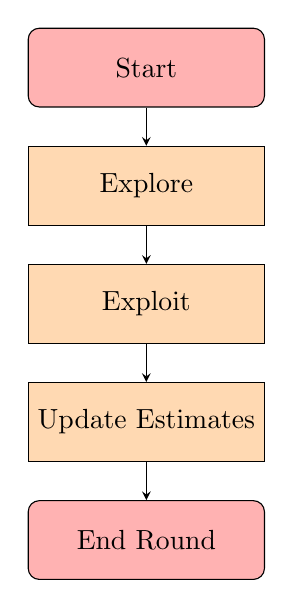
\begin{tikzpicture}[node distance=1cm, >=stealth]
        \node (start) [startstop] {Start};
        \node (explore) [process, below of=start, yshift=-0.5cm] {Explore};
        \node (exploit) [process, below of=explore, yshift=-0.5cm] {Exploit};
        \node (update) [process, below of=exploit, yshift=-0.5cm] {Update Estimates};
        \node (end) [startstop, below of=update, yshift=-0.5cm] {End Round};
        
        \draw[->] (start) -- (explore);
        \draw[->] (explore) -- (exploit);
        \draw[->] (exploit) -- (update);
        \draw[->] (update) -- (end);
    \end{tikzpicture}
\end{columns}
\end{frame}

\section{BGA: Pseudocode Overview}

\begin{frame}
\frametitle{Pseudocode for BGA Algorithm}
\begin{block}{BGA Algorithm}
\begin{enumerate}
    \item Initialize estimates and sampling basis \( B \subset S \).
    \item For each round \( t = 1 \) to \( T \):
    \begin{enumerate}
        \item With probability \( \gamma \), \textbf{explore} by selecting a random basis vector \( b \in B \).
        \item Otherwise, \textbf{exploit} by selecting \( x_t \) using the Kalai-Vempala strategy on estimated costs.
        \item Observe the incurred cost \( c_t \cdot x_t \).
        \item Update cost estimates based on the observed cost.
    \end{enumerate}
\end{enumerate}
\end{block}
\begin{exampleblock}{Flowchart Representation}
    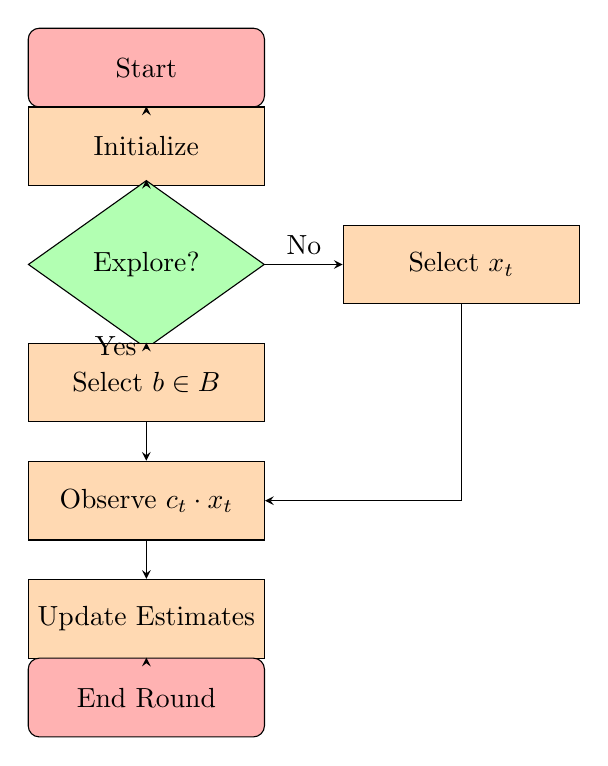
\begin{tikzpicture}[node distance=1cm, >=stealth, auto]
        \node (start) [startstop] {Start};
        \node (init) [process, below of=start] {Initialize};
        \node (decide) [decision, below of=init, yshift=-0.5cm] {Explore?};
        \node (explore) [process, below of=decide, yshift=-0.5cm] {Select \( b \in B \)};
        \node (exploit) [process, right of=decide, xshift=3cm] {Select \( x_t \)};
        \node (observe) [process, below of=explore, yshift=-0.5cm] {Observe \( c_t \cdot x_t \)};
        \node (update) [process, below of=observe, yshift=-0.5cm] {Update Estimates};
        \node (end) [startstop, below of=update] {End Round};
        
        \draw[->] (start) -- (init);
        \draw[->] (init) -- (decide);
        \draw[->] (decide) -- node[anchor=east] {Yes} (explore);
        \draw[->] (decide) -- node[anchor=south] {No} (exploit);
        \draw[->] (explore) -- (observe);
        \draw[->] (exploit) |- (observe);
        \draw[->] (observe) -- (update);
        \draw[->] (update) -- (end);
    \end{tikzpicture}
\end{exampleblock}
\end{frame}

\section{The Role of Basis \( B \) in BGA}

\begin{frame}
\frametitle{Explanation of the Sampling Basis \( B \subset S \)}
\begin{itemize}
    \item \( B \) is a carefully chosen subset of \( S \) that facilitates exploration.
    \item Ensures coverage of different regions in the decision space.
    \item Basis vectors are used to approximate the cost structure.
    \item Geometric properties of \( B \) influence the efficiency of exploration.
\end{itemize}
\begin{exampleblock}{Mathematical Insight}
    If \( B \) forms a \textbf{basis} in the linear algebra sense, any decision \( x \in S \) can be expressed as a linear combination of vectors in \( B \). This allows efficient reconstruction and estimation of the cost vector \( c_t \).
\end{exampleblock}
\end{frame}

\begin{frame}
\frametitle{Decision Making Based on Basis \( B \)}
\begin{itemize}
    \item During exploration, a basis vector \( b \) is selected uniformly at random.
    \item Provides unbiased estimates of the cost vector \( c_t \).
    \item Facilitates efficient updating of cost estimates.
\end{itemize}
\begin{equation*}
    \hat{c}_t = \frac{c_t \cdot b}{P(b)} e_b
    \end{equation*}
    where \( P(b) \) is the probability of selecting basis vector \( b \), and \( e_b \) is the corresponding basis vector.
\end{frame}

\section{Exploration vs. Exploitation}

\begin{frame}
\frametitle{Exploration Probability \( \gamma \)}
\begin{itemize}
    \item \( \gamma \) controls the frequency of exploration.
    \item Higher \( \gamma \) leads to more exploration, improving cost estimates.
    \item Lower \( \gamma \) emphasizes exploitation, leveraging current knowledge.
\end{itemize}
\begin{block}{Balancing \( \gamma \)}
    The optimal choice of \( \gamma \) depends on problem parameters such as \( T \) and \( n \). Typically, \( \gamma \) is set to decrease over time to balance exploration and exploitation effectively.
\end{block}
\end{frame}

\begin{frame}
\frametitle{Trade-off Between Exploration and Exploitation}
\begin{columns}
    \column{0.6\textwidth}
    \begin{itemize}
        \item Balancing \( \gamma \) is crucial for minimizing regret.
        \item Too much exploration can waste resources, while too little can lead to poor estimates.
        \item Optimal \( \gamma \) depends on problem parameters like \( T \) and \( n \).
    \end{itemize}
    \column{0.4\textwidth}
    % \includegraphics[width=\textwidth]{images/exploration_exploitation_tradeoff.png} % Replace with your image path
\end{columns}
\end{frame}

\section{Estimate Update and Matrix Inversion}

\begin{frame}
\frametitle{Update Rule for Cost Vector Estimates}
\begin{itemize}
    \item Use observed costs to refine estimates of \( c_t \).
    \item Employ matrix inversion techniques to handle correlated estimates.
    \item Ensures accurate approximation of the true cost vectors over time.
    \item Utilizes geometric properties of the decision set for efficient updates.
\end{itemize}
\begin{equation*}
    \hat{c}_{t+1} = \hat{c}_t - \eta \nabla L_t(x_t)
\end{equation*}
where \( \eta \) is the learning rate and \( L_t(x_t) \) is the loss at round \( t \).
\end{frame}

\section{Mathematical Setup for Analysis}

\begin{frame}
\frametitle{Introduction to the Mathematical Analysis of BGA}
\begin{itemize}
    \item Formalize the algorithm's update rules and decision-making process.
    \item Define assumptions and properties of the cost vectors and decision set.
    \item Set the stage for deriving regret bounds.
\end{itemize}
\begin{exampleblock}{Assumptions}
    \begin{enumerate}
        \item The cost vectors \( c_t \) are bounded, i.e., \( \|c_t\| \leq C \) for some constant \( C \).
        \item The decision set \( S \) is convex and compact.
        \item The adversary is adaptive, choosing \( c_t \) based on past decisions \( x_1, \dots, x_{t-1} \).
    \end{enumerate}
\end{exampleblock}
\end{frame}

\begin{frame}
\frametitle{Regret Bounds and Performance Guarantees}
\begin{columns}
    \column{0.6\textwidth}
    \begin{itemize}
        \item Analyze the cumulative regret over \( T \) rounds.
        \item Provide theoretical guarantees under adaptive adversary models.
        \item Compare performance with existing algorithms like Kalai-Vempala.
    \end{itemize}
    \column{0.4\textwidth}
    % \includegraphics[width=\textwidth]{images/regret_analysis.png} % Replace with your image path
\end{columns}
\begin{block}{Theoretical Insight}
    Under the adaptive adversary model, BGA maintains a regret bound of:
    \[
    \text{Regret} = O\left(T^{3/4} \sqrt{\ln T}\right)
    \]
    This ensures that the algorithm performs competitively even in dynamic environments.
\end{block}
\end{frame}

\section{Bounds on Regret}

\begin{frame}
\frametitle{Theoretical Regret Result}
\begin{itemize}
    \item BGA achieves regret \( O\left(T^{3/4} \sqrt{\ln T}\right) \).
    \item Sublinear growth ensures that average regret per round diminishes.
    \item Demonstrates effectiveness in the bandit setting against adaptive adversaries.
\end{itemize}
\begin{block}{Mathematical Proof Sketch}
    The regret bound is derived using:
    \begin{enumerate}
        \item Concentration inequalities to bound estimation errors.
        \item Matrix inversion to handle dependencies in cost estimates.
        \item Balancing exploration and exploitation through parameter tuning.
    \end{enumerate}
\end{block}
\end{frame}

\begin{frame}
\frametitle{Impact of Parameters \( \gamma \), \( \epsilon \), and \( T \)}
\begin{itemize}
    \item \( \gamma \): Balances exploration and exploitation.
    \item \( \epsilon \): Determines precision of cost estimates.
    \item \( T \): Number of rounds influences overall regret.
    \item Optimal tuning of parameters is essential for best performance.
\end{itemize}
\begin{equation*}
    \gamma = T^{-1/4}, \quad \epsilon = T^{-1/2}
\end{equation*}
\end{frame}

\section{High Probability Bounds}

\begin{frame}
\frametitle{High-Probability Bounds on Cost Vector Estimates}
\begin{itemize}
    \item Establish bounds that hold with high probability.
    \item Use concentration inequalities to ensure reliable estimates.
    \item Critical for guaranteeing low regret in adversarial settings.
\end{itemize}
\begin{equation*}
    \Pr\left( \|\hat{c}_t - c_t\| \geq \delta \right) \leq \exp(-k\delta^2)
\end{equation*}
where \( k \) is a constant depending on \( T \) and \( n \).
\end{frame}

\begin{frame}
\frametitle{Using Martingale Inequalities for Estimating \( c_t \)}
\begin{itemize}
    \item Apply martingale-based techniques to handle dependencies over time.
    \item Ensure that estimates remain unbiased and concentrated around true values.
    \item Facilitates robust analysis against adaptive adversaries.
\end{itemize}
\begin{theorem}[Azuma-Hoeffding Inequality]
    Let \( \{X_t\} \) be a martingale with bounded differences \( |X_t - X_{t-1}| \leq c_t \). Then, for any \( \lambda > 0 \),
    \[
    \Pr\left( X_T - X_0 \geq \lambda \right) \leq \exp\left( -\frac{\lambda^2}{2 \sum_{t=1}^T c_t^2} \right)
    \]
\end{theorem}
\end{frame}

\section{Exploration of Basis and Estimation}

\begin{frame}
\frametitle{Random Exploration for Estimating True Cost Vectors}
\begin{itemize}
    \item Randomly selecting basis vectors aids in uncovering the cost structure.
    \item Ensures diverse coverage of the decision space.
    \item Reduces bias in cost estimates by providing varied perspectives.
\end{itemize}
\begin{equation*}
    \mathbb{E}[\hat{c}_t] = c_t
\end{equation*}
\begin{block}{Unbiased Estimation}
    The estimator \( \hat{c}_t \) is unbiased because:
    \[
    \mathbb{E}[\hat{c}_t] = \sum_{b \in B} P(b) \cdot \frac{c_t \cdot b}{P(b)} e_b = c_t
    \]
\end{block}
\end{frame}

\begin{frame}
\frametitle{Importance of Unbiased Estimates}
\begin{itemize}
    \item Unbiased estimates are crucial for accurate decision-making.
    \item Prevents systematic errors that could be exploited by the adversary.
    \item Enhances the reliability and performance of the BGA algorithm.
\end{itemize}
\begin{equation*}
    \mathbb{E}[\hat{c}_t] = c_t
\end{equation*}
\begin{block}{Consequence}
    Ensures that the algorithm's decisions are based on accurate representations of the cost vectors, leading to effective optimization over time.
\end{block}
\end{frame}

\section{Performance Bound: Expected Regret}

\begin{frame}
\frametitle{Detailed Analysis of Expected Regret for BGA}
\begin{itemize}
    \item Derive bounds on the expected cumulative regret.
    \item Show how BGA maintains low regret despite adaptive adversaries.
    \item Compare theoretical performance with empirical observations.
\end{itemize}
\begin{block}{Expected Regret Bound}
    The expected regret of BGA satisfies:
    \[
    \mathbb{E}[\text{Regret}] \leq O\left(T^{3/4} \sqrt{\ln T}\right)
    \]
    \begin{itemize}
        \item The bound holds under the adaptive adversary model.
        \item Demonstrates sublinear growth, ensuring diminishing average regret.
    \end{itemize}
\end{block}
\end{frame}

\section{Summary of Theoretical Results}

\begin{frame}
\frametitle{Summary of Performance Guarantees}
\begin{itemize}
    \item BGA achieves sublinear regret in the bandit setting.
    \item Provides robustness against adaptive adversaries.
    \item Maintains competitive performance compared to full-information algorithms.
\end{itemize}
\begin{block}{Key Takeaways}
    \begin{itemize}
        \item Sublinear regret ensures that the algorithm becomes more effective over time.
        \item Robustness against adaptive adversaries makes BGA suitable for dynamic environments.
        \item The bandit setting presents unique challenges that BGA effectively addresses.
    \end{itemize}
\end{block}
\end{frame}

\begin{frame}
\frametitle{Comparison with Kalai-Vempala Algorithm}
\begin{itemize}
    \item Kalai-Vempala assumes full feedback, achieving different regret bounds.
    \item BGA extends these ideas to the bandit setting with limited feedback.
    \item Demonstrates comparable performance with additional challenges.
\end{itemize}
\begin{table}[h]
\centering
\begin{tabular}{|l|c|c|}
\hline
\textbf{Algorithm} & \textbf{Feedback} & \textbf{Regret Bound} \\ \hline
Kalai-Vempala & Full Information & \( O(\sqrt{T}) \) \\ \hline
BGA & Bandit & \( O(T^{3/4} \sqrt{\ln T}) \) \\ \hline
\end{tabular}
\caption{Comparison of Regret Bounds}
\end{table}
\end{frame}

\section{Conclusions}

\begin{frame}
\frametitle{Recap of the Main Contribution}
\begin{itemize}
    \item Introduction of BGA for online geometric optimization in bandit settings.
    \item Achieves low-regret performance against adaptive adversaries.
    \item Bridges the gap between full-information and bandit feedback models.
\end{itemize}
\begin{block}{Implications}
    BGA provides a robust framework for decision-making in environments where feedback is limited and adversaries can adapt, making it applicable to various real-world scenarios.
\end{block}
\end{frame}

\begin{frame}
\frametitle{Theoretical Bounds for Performance Against an Adaptive Adversary}
\begin{itemize}
    \item Established \( O(T^{3/4} \sqrt{\ln T}) \) regret bound.
    \item Guarantees hold under general adversarial conditions.
    \item Highlights the algorithm's robustness and efficiency.
\end{itemize}
\begin{block}{Future Directions}
    Further research can explore tightening these bounds and extending BGA to other optimization settings.
\end{block}
\end{frame}

\section{Open Problems}

\begin{frame}
\frametitle{Discussion of Open Questions and Potential Future Work}
\begin{itemize}
    \item Can regret bounds be further improved for adaptive adversaries?
    \item Exploration of different sampling strategies for basis selection.
    \item Extensions to other types of online optimization problems.
    \item Incorporating additional feedback mechanisms to enhance performance.
\end{itemize}
\end{frame}

\begin{frame}
\frametitle{Improving Regret Bounds for Adaptive Adversaries}
\begin{itemize}
    \item Investigate tighter analyses and alternative algorithms.
    \item Explore the impact of different geometric properties of \( S \).
    \item Consider hybrid models combining full and bandit feedback.
    \item Study the interplay between exploration rates and adversary adaptability.
\end{itemize}
\begin{block}{Potential Approaches}
    \begin{enumerate}
        \item Utilize advanced concentration inequalities.
        \item Incorporate adaptive learning rates.
        \item Leverage multi-armed bandit techniques.
    \end{enumerate}
\end{block}
\end{frame}

\section{References}

\begin{frame}
\frametitle{Key References}
\begin{itemize}
    \item Kalai, E., \& Vempala, S. (2005). A polynomial time algorithm for online convex programming. \textit{Proceedings of the ACM Conference on Learning Theory}, 161-170.
    \item McMahan, H. B., \& Blum, A. (Year). \textit{Title of the Paper}. \textit{Journal/Conference Name}.
    \item Auer, P., Cesa-Bianchi, N., \& Fischer, P. (2002). Finite-time Analysis of the Multiarmed Bandit Problem. \textit{Machine Learning}, 47(2-3), 235-256.
    \item [Additional relevant literature on online optimization and bandit algorithms.]
\end{itemize}
\end{frame}

\section{Acknowledgments}

\begin{frame}
\frametitle{Acknowledgments}
\begin{itemize}
    \item Thank collaborators and contributors.
    \item Acknowledge funding sources and institutional support.
    \item Express gratitude to reviewers and advisors.
\end{itemize}
\begin{block}{Example}
    We would like to thank our colleagues at Carnegie Mellon University for their invaluable feedback and support. This work was supported by NSF Grant \#XXXXXX.
\end{block}
\end{frame}

\end{document}
